\title{Media streaming models}

\maketitle
\tableofcontents

\section{Single Layer Coding (SLC) + Client/Server (C/S) Model}
%{{{

\fig{400}{SLC+CS.png}

\begin{itemize}
\item Notice that a buffer underflow (i.e. a lost of a GOP during the
  playback) can occur if $t_T<t_E$ (the transmission bit-rate is smaller
  than the encoding bit-rate).
\end{itemize}

%}}}

\section{Media simulcast + Client/Server (C/S) Model}
%{{{

\fig{400}{simulcast+CS.png}

\begin{itemize}
\item If the client's buffer is going to underflow, the client should
  retrieve a stream with a smaller bit-rate (this happens for the
  GOP$_2$).
\end{itemize}
% \item In a solution to provide service scalability, a media server can
%   store (and serve) collection of non-scalable streams, depending on
%   the characteristics of the transmission channel and the receiver
%   (resolution, computing power, battery, etc.). Notice that
%   simulcasting produces a replication of information at the server
%   side, but not on the network nor the clients.
% \item This is used, for example, at YouTube.
% \item Currently, most video servers provide spatial scalability
%   (YouTube, for example) by means of media simulcast. However, due to
%   stream switching is not supported by the Web browsers along the
%   playing, the selection of the resolution must be done only at the
%   beginning of the transmission.
% \item Moreover, temporal and quality scalabilities are not supported
%   by current Web browsers because only single-layer (non-scalable)
%   decoders are implemented in them, even when the GOPs (that could
%   change the picture-rate or the quality) can be decoded
%   independently.
% \item However, notice that this is only a lack of functionality of the
%   majority of the browsers. This could be solved soon.

%}}}

\section{Multiple Layer Coding (MLC) + Client/Server (C/S) Model}
%{{{

\fig{400}{MLC+CS.png}
\begin{center}
  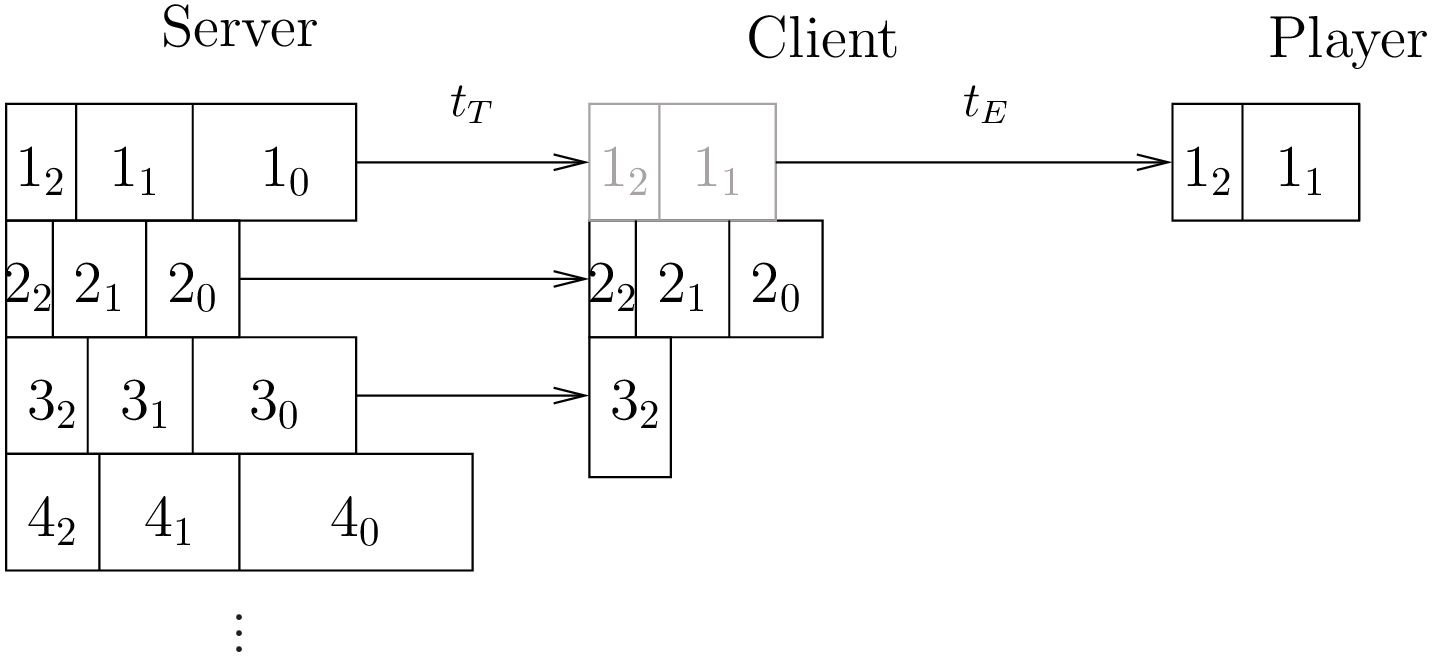
\includegraphics[width=0.8\textwidth]{MLC+CS}
\end{center}

\begin{itemize}
\item If the client's buffer is going to underflow, the client should
  retrieve less layers.
\end{itemize}

%}}}

\section{Multiple Description Coding (MDC) + Client/Server (C/S) Model}
%{{{

\fig{400}{MDC+CS.png}

\begin{itemize}
\item If the client's buffer is going to underflow, the client should
  retrieve less descriptions (this happens for the GOP$_2$).
\end{itemize}

%}}}

\section{Single Layer Coding (SLC) + Peer-to-Peer (P2P) Model}
%{{{

\begin{itemize}
\item Due to all peers need to share the same single-layered stream,
  $t_E$ should never be bigger than $t_T$, for every peer in the cluster,
  or a buffer underflow will occur in those peers where $t_E>t_T$.
\end{itemize}

%}}}

\section{Media simulcast + Peer-to-Peer (P2P) Model}
%{{{

\begin{itemize}
\item Each media can be simultaneously broadcasted but in different
  channels (clusters of peers).
\item Peers can switch between clusters depending on the transmission
  bit-rate (channel switching should be fast in order to use
  efficiently the available bandwidth).
\item The time to perform a switch between channels depends on the
  buffering time.
%, which depends on the buffer size, the transmission
%  bit-rate and the GOP-rate, that depends on the GOP size and the
%  picture-rate.
%\item In a switch, the end of the reception of the old channel should
%  coincide with the beginning of the reception of the new channel,
%  i.e, the buffering time should be predictable. Otherwise, the
%  reception of both channels must be overlapped.
% \item Due to all peers need to share the same simulcasted stream, only
%   a high bit-rate GOP should be delivered by the source if all peers
%   can receive such amount of data.
\end{itemize}

%}}}

\section{Multiple Layer Coding (MLC) + Peer-to-Peer (P2P) Model}
%{{{

\begin{itemize}
\item If each layer is transmitted over a different cluster, peers can
  join/left to more/less clusters depending on the transmission
  bit-rate.
\item The transmission of the layer $X-1$ must be prioritized to the
  transmission of the layer $X$.
% \item Because the $X$-th quality, resolution or picture-rate implies
%   the reception of all layers up to the the $X$-th one, all peers can
%   share the same scalable stream independently of the number of layers
%   received.
\end{itemize}

%}}}

\section{Multiple Description Coding (MDC) + Peer-to-Peer (P2P) Model}
%{{{

\begin{itemize}
\item As in MLC, if each description is transmitted over a different
  cluster, peers can join/left to more/less clusters depending on the
  transmission bit-rate.
\item However, in this case it is not necessary to prioritize the
  transmission of the descriptions (although a peer could be rejected
  from a cluster (description) if it becomes unsupportive).
\end{itemize}

%}}}

